%%%%%%%%%%%%%%%%%%%%%%%%%%%%%%%%%%%%
% Header                           %
%%%%%%%%%%%%%%%%%%%%%%%%%%%%%%%%%%%%
%
% Compilation:
%
% - with pdfLaTeX:
%   pdflatex -> biber -> makeindex/create_glossaries.cmd -> pdflatex -> pdflatex
% - For compilation add switch -shell-escape in your LaTeX editor:
%   pdflatex --shell-escape -synctex=1 -interaction=nonstopmode %source --extra-mem-top=60000000
% - Compile at least 3 times for proper output
%
% In case of problems:
%
% - Increase Tex-Memory in batch with:
%   initexmf --edit-config-file pdflatex
%   add: main_memory=8000000
%   initexmf --dump=pdflatex
%
% Revisions: 2017-04-10 Martin R�del <martin.raedel@dlr.de>
%                       Initial draft
%
% Contact:   Martin R�del,  martin.raedel@dlr.de
%            DLR Composite Structures and Adaptive Systems
%
%                                 __/|__
%                                /_/_/_/  
%            www.dlr.de/fa/en      |/ DLR
% 
%%%%%%%%%%%%%%%%%%%%%%%%%%%%%%%%%%%%

% ---------------------------
% Paths
% ---------------------------

\newcommand{\peridoccommonpath}{../PeriDoX_Common}
\newcommand{\peridocliteraturepath}{../../Literature}

% ---------------------------
% Documentclass
% ---------------------------

\documentclass[%
  figures=plain,%
  listof=totoc,%                                % List of figures, tables in TOC
  bibliography=totoc,%                          % Bibliography in TOC
  %index=totoc,                                  % Index in TOC
  fleqn,%                                       % left-align equations
% ]{dlrreprt}                                     % Full dlrreprt.class with Frutiger font
]{bootstrap_dlrreprt}                           % Bootstrap of dlrreprt without Frutiger font
%
%%%%%%%%%%%%%%%%%%%%%%%%%%%%%%%%%%%%
% Preamble                         %
%%%%%%%%%%%%%%%%%%%%%%%%%%%%%%%%%%%%

% ---------------------------
% Path to common
% ---------------------------

\newcommand{\peridoccommonpath}{../../../../Doc/PeriDoX_Common}
\newcommand{\peridocliteraturepath}{../../../../Literature}
\newcommand{\materialpath}{../../Material}

% ---------------------------
% Local packages
% ---------------------------

\usepackage[
  style=numeric-comp,
  sorting=none,
  url=false,
  isbn=false
]{biblatex}
\usepackage{booktabs}
\usepackage{caption}
\usepackage{enumitem}
\usepackage{filecontents}
\usepackage{multirow}
% \usepackage{placeins} % for \FloatBarrier
\usepackage{siunitx}
\sisetup{%
  exponent-product = \cdot,%
  output-product = \cdot,%
  separate-uncertainty=true,% uncertainty is separated with a "plus-minus" symbol
}
\usepackage{subcaption}
\usepackage{tabularx}

% General preamble
% %%%%%%%%%%%%%%%%%%%%%%%%%%%%%%%%%%%%
% Header                           %
%%%%%%%%%%%%%%%%%%%%%%%%%%%%%%%%%%%%
% 
% This file handles all things with general packages
% 
% Revisions: 2017-04-10 Martin Raedel <martin.raedel@dlr.de>
%                       Initial draft
%               
% Contact:   Martin Raedel,  martin.raedel@dlr.de
%            DLR Composite Structures and Adaptive Systems
%          
%                                 __/|__
%                                /_/_/_/  
%            www.dlr.de/fa/en      |/ DLR
% 
%%%%%%%%%%%%%%%%%%%%%%%%%%%%%%%%%%%%
% Content                          %
%%%%%%%%%%%%%%%%%%%%%%%%%%%%%%%%%%%%

% ---------------------------
% Packages
% ---------------------------

% Every package with the exception of
% - RMLaTeX-packages
% - Hyperref
% - Every package that has to be placed after hyperref -> Pref_Packages_Hyperref.tex
\usepackage[latin1]{inputenx}
\usepackage[T1]{fontenc}
\usepackage{amsmath}
\usepackage{amssymb}
\usepackage{amsthm}
\usepackage[page,titletoc]{appendix}
\usepackage{array}
% babel package is loaded seperately. Allows reuse for projects with various languages
% biblatex package is loaded in Pref_BibLaTeX_XYZ.tex from PeriDoc_Common
\usepackage{booktabs}
\usepackage{caption}
\usepackage{calc}
\usepackage{color}
\usepackage{coseoul}
\usepackage{csquotes}
\usepackage{enumitem}
\usepackage{esvect}
\usepackage{etoolbox}
\usepackage{filecontents}
% http://tex.stackexchange.com/a/312910/44634 for fixing clash between filecontents and morewrites
\newwrite\fcwrite
\makeatletter
\let\zzzz\filec@ntents
\def\filec@ntents{\def\chardef##1\write{\let\reserved@c\fcwrite}\zzzz}
\makeatother
% Mute "Overwriting file" warning for filecontents package
\usepackage{ifthen}
\usepackage{ltxtable}
\usepackage{marginnote}
\usepackage{marvosym}                            % Symbols: \Faxmachine, \Mundus, \Letter
\usepackage{mathtools}
\usepackage{media9}
\usepackage{morewrites}                          % http://tex.stackexchange.com/q/289734
\usepackage{multicol}
\usepackage{multirow}
%\usepackage{nomencl}
\usepackage{pifont}
\usepackage{placeins}
\usepackage{subcaption}
\usepackage{tabto}
\usepackage{tabu}
\usepackage{tabularx}
\usepackage[most]{tcolorbox}
\usepackage{textcomp}

\makeatletter
\@ifundefined{KOMAClassName}
  {% true -> no KOMA class
    \@ifclassloaded{amsart}{
      % Do nothing! Amsart does not play with titlesec package
    }{
      \usepackage{titlesec}    
    }
  }
  {% false -> KOMA class
  }
\makeatother

\usepackage[figure,table,lstlisting]{totalcount}
\usepackage{upquote}
\usepackage{wasysym}                            % Symbols \& Smileys :)
\usepackage{wrapfig}
\usepackage{xparse}

\usepackage{hyphenat}
% %%%%%%%%%%%%%%%%%%%%%%%%%%%%%%%%%%%%
% Header                           %
%%%%%%%%%%%%%%%%%%%%%%%%%%%%%%%%%%%%
% 
% This file handles all things considering the hyperref package
%
% Requirements:
%
% - use of either Pref_Language_English.tex or Pref_Language_German.tex before this file
% 
% Revisions: 2017-04-10 Martin Raedel <martin.raedel@dlr.de>
%                       Initial draft
%               
% Contact:   Martin Raedel,  martin.raedel@dlr.de
%            DLR Composite Structures and Adaptive Systems
%          
%                                 __/|__
%                                /_/_/_/  
%            www.dlr.de/fa/en      |/ DLR
% 
%%%%%%%%%%%%%%%%%%%%%%%%%%%%%%%%%%%%
% Content                          %
%%%%%%%%%%%%%%%%%%%%%%%%%%%%%%%%%%%%

% ---------------------------
% Load package
% ---------------------------

% https://tex.stackexchange.com/questions/17218/make-hyperref-take-pdfinfo-from-title-and-author
\makeatletter
\@ifpackageloaded{hyperref}{}{
  \usepackage[%
    % These options must be set at the time of \usepackage and can not be set using \hypersetup
    bookmarks = true,
    pdfusetitle,%
  ]{hyperref}
}
\makeatother

% ---------------------------
% Package options
% ---------------------------

\makeatletter%
  \@ifclassloaded{elsarticle}{}{% elsarticle works with natbib instead of BibLaTeX
    \hypersetup{%
      colorlinks = true,%
      linkcolor  = black,%
      citecolor  = black,%
      urlcolor   = blue,%
      pdfstartview = Fit,%
      pdfmenubar = true,%
      pdftoolbar = true,%
      %
      bookmarksopen = false,
      %bookmarksopenlevel = 1,
    }
  }
\makeatother

% ---------------------------
% Renewcommand hyperref autorefnames
% ---------------------------

%cross references to equations with parenthesis
%\newcommand{\RefEq}[1]{\equationautorefname~\eqref{#1}}

%cross references to figures
%\newcommand{\RefFig}[1]{\figureautorefname~\ref{#1}}

%cross references to tables
%\newcommand{\RefTab}[1]{\tableautorefname~\ref{#1}}

% http://tex.stackexchange.com/questions/36575/autorefs-inserted-text-has-not-the-correct-case
\iflanguage{english}{
  \AtBeginDocument{
    \renewcommand*{\equationautorefname}{Equation}
    \renewcommand*{\figureautorefname}{Figure}
    \renewcommand*{\tableautorefname}{Table}
  }
}

\iflanguage{ngerman}{
  \AtBeginDocument{
    \renewcommand*{\equationautorefname}{Gleichung}
    \renewcommand*{\figureautorefname}{Abbildung}
    \renewcommand*{\tableautorefname}{Tabelle}
  }
}

% ---------------------------
% Packages after Hyperref
% ---------------------------

\usepackage{attachfile}
%%%%%%%%%%%%%%%%%%%%%%%%%%%%%%%%%%%%
% Header                           %
%%%%%%%%%%%%%%%%%%%%%%%%%%%%%%%%%%%%
% 
% This file handles all things considering the siunitx package
%
% Revisions: 2016-03-06 Martin Raedel <martin.raedel@dlr.de>
%                       Initial draft
%               
% Contact:   Martin Raedel,  martin.raedel@dlr.de
%            DLR Composite Structures and Adaptive Systems
%          
%                                 __/|__
%                                /_/_/_/  
%            www.dlr.de/fa/en      |/ DLR
% 
%%%%%%%%%%%%%%%%%%%%%%%%%%%%%%%%%%%%
% Content                          %
%%%%%%%%%%%%%%%%%%%%%%%%%%%%%%%%%%%%

%-----------------------------------
% Load package
%-----------------------------------

\usepackage{siunitx}

%-----------------------------------
% Setup
%-----------------------------------

\sisetup{%
  exponent-product = \cdot,%
  output-product = \cdot,%
  binary-units=true,%
}

%-----------------------------------
% New units
%-----------------------------------

% Length
\DeclareSIUnit\foot{ft}
\DeclareSIUnit\inch{in}

% Temperature
\DeclareSIUnit\degreeFahrenheit{^{\circ}F}
\DeclareSIUnit\degreeRankine{^{\circ}R}

% Force
\DeclareSIUnit\dyn{dyn}
\DeclareSIUnit\poundforce{lbf}

% Pressure
\DeclareSIUnit\barye{Ba}
\DeclareSIUnit\psi{psi}

% Density
\DeclareSIUnit\slug{slug}

% Energy
\DeclareSIUnit\erg{erg}

% Promille
\DeclareSIUnit[number-unit-product = \,]{\promille}{\textperthousand}
%%%%%%%%%%%%%%%%%%%%%%%%%%%%%%%%%%%%
% Header                           %
%%%%%%%%%%%%%%%%%%%%%%%%%%%%%%%%%%%%
% 
% This file handles all things considering the TikZ package
%
% Revisions: 2016-03-06 Martin Raedel <martin.raedel@dlr.de>
%                       Initial draft
%               
% Contact:   Martin Raedel,  martin.raedel@dlr.de
%            DLR Composite Structures and Adaptive Systems
%          
%                                 __/|__
%                                /_/_/_/  
%            www.dlr.de/fa/en      |/ DLR
% 
%%%%%%%%%%%%%%%%%%%%%%%%%%%%%%%%%%%%
% Content                          %
%%%%%%%%%%%%%%%%%%%%%%%%%%%%%%%%%%%%

% ---------------------------
% Load package
% ---------------------------

\makeatletter
\@ifpackageloaded{tikz}{
  %\usetikzlibrary{angles}
  \usetikzlibrary{arrows.meta}
  \usetikzlibrary{backgrounds}
  \usetikzlibrary{calc}
  \usetikzlibrary{decorations.markings}
  \usetikzlibrary{decorations.text}
  \usetikzlibrary{fit}
  % \usetikzlibrary{fpu}
  \usetikzlibrary{intersections}
  \usetikzlibrary{tikzmark}
  \usetikzlibrary{trees}
  \usetikzlibrary{matrix}
  \usetikzlibrary{patterns}
  \usetikzlibrary{positioning}
  \usetikzlibrary{shadows}
  % \usetikzlibrary{shapes}
  \usetikzlibrary{shapes.misc}
  \usetikzlibrary{spy}
}{
  \usepackage{tikz}
  %\usetikzlibrary{angles}
  \usetikzlibrary{arrows.meta}
  \usetikzlibrary{backgrounds}
  \usetikzlibrary{calc}
  \usetikzlibrary{decorations.markings}
  \usetikzlibrary{decorations.text}
  \usetikzlibrary{fit}
  % \usetikzlibrary{fpu}
  \usetikzlibrary{intersections}
  \usetikzlibrary{tikzmark}
  \usetikzlibrary{trees}
  \usetikzlibrary{matrix}
  \usetikzlibrary{patterns}
  \usetikzlibrary{positioning}
  \usetikzlibrary{shadows}
  % \usetikzlibrary{shapes}
  \usetikzlibrary{shapes.misc}
  \usetikzlibrary{spy}
}
\makeatother

% ---------------------------
% Pgfmath
% ---------------------------

\makeatletter
% Stuff for calc compatiability.
\let\real=\pgfmath@calc@real
\let\minof=\pgfmath@calc@minof
\let\maxof=\pgfmath@calc@maxof
\let\ratio=\pgfmath@calc@ratio
\let\widthof=\pgfmath@calc@widthof
\let\heightof=\pgfmath@calc@heightof
\let\depthof=\pgfmath@calc@depthof
\makeatother

% ---------------------------
% Tikzsets
% ---------------------------

% Default arrow tip
\tikzset{
  defarrow/.style={                           % Define arrow style
    >=Stealth,                                % >=latex
  }
}

\tikzset{
  every picture/.style=semithick              % Adjust default line width
}

% Help grid for external images
% Call inside scope with: \pic{myimagegrid};
\tikzset{%
  myimagegrid/.pic={%
   \draw[help lines,xstep=.1,ystep=.1] (0,0) grid (1,1);
   \foreach \x in {0,1,...,9} {\node [anchor=north] at (\x/10,0) {0.\x};}
   \foreach \y in {0,1,...,9} {\node [anchor=east]  at (0,\y/10) {0.\y};}
  }%
}

% Equal space decoration markers along addplot path
% http://tex.stackexchange.com/a/232010/44634
\makeatletter
\tikzset{
  nomorepostactions/.code={\let\tikz@postactions=\pgfutil@empty},
  mymark/.style 2 args={decoration={markings,
    mark= between positions 0 and 1 step (1/11)*\pgfdecoratedpathlength with{%
        \tikzset{#2,every mark}\tikz@options
        \pgfuseplotmark{#1}%
      },  
    },
    postaction={decorate},
    /pgfplots/legend image post style={
      mark=#1,
      #2,
      every path/.append style={nomorepostactions}
    },
  },
}
\makeatother

% Markup style for rectangles on external figures
% Needs Pref_Color.tex for mymarkupcolor
\tikzset{%
  myrectangularmarkup/.style={%
   inner sep=0pt,% necessary for correct positioning of corners
   draw=mymarkupcolor,%
   thick,%
  }%
}

\tikzset{%
  mymarkuptext/.style={%
   text=mymarkupcolor,%
  }%
}

% A croos for markings in plots
% https://tex.stackexchange.com/a/124064
\tikzset{cross/.style={cross out, draw, 
         minimum size=2*(#1-\pgflinewidth), 
         inner sep=0pt, outer sep=0pt}}

% ---------------------------
% Pgfkeys
% ---------------------------

% From the pgf manual 2.10csv page 694:
% 
%     It should be noted that all calculations must not exceed �16383.99999 at any point, because the underlying computations rely on TeX dimensions. This means that many of the underlying computations are necessarily approximate and that in addition, are not very fast. TeX is, after all, a typesetting language and not ideally suited to relatively advanced mathematical operations. However, it is possible to change the computations as described in Section 76.
% 
% From the TeX Book page 114:
% 
%     16383.99998pt (TeX's largest dimen)
% 
% In Notes On Programming in TeX Chirstian Feuersaenger pointed out
% 
%     The \dimen registers perform their arithmetic's internally with 32 bit scaled integers, so called scaled point with unit sp. It holds 1pt = 65536sp = 216sp. One of the 32 bits is used as sign. The total number range in pt is [-(2^30-1)/2^16,(2^30-1)/2^16 ]=[-16383.9998, +16383.9998]1.
% 
%     1 Please note that this does not cover the complete range of a 32 bit integer, I do not know why
% \pgfkeys{/pgf/fpu=true}                       % Allow pgf to plot values larger than 16383.9998
% \tikzset{fpu}                                   % Allow pgf to plot values larger than 16383.9998

\pgfkeys{/tikz/savenumber/.code 2 args={\global\edef#1{#2}}}

% ---------------------------
% tikzsets
% ---------------------------

%~~~~~ WaveChart Style ~~~~~~~~~~

\tikzset{
  wavespy style/.style={
    spy scope={%
      wavespyscope style,%
    },
    connect spies/.style={
      wavespyconnect style,%
    },
  }
}

\tikzset{
  wavespyscope style/.style={
    magnification=4,
    connect spies,                            % Connect orig. & detail
    width=2.0cm,                              % Spy width
    height=1.0cm,                             % Spy height
    every spy on node/.style={                % Source
      rectangle,                              % Form
      rounded corners,                        % Edge shape
      dashed,                                 % Dashed line
      draw=gray,                              % Line color
      thick,                                  % Line style for spy
    },
    every spy in node/.style={                % Spy
      rectangle,                              % Form
      rounded corners,                        % Edge shape
      dashed,                                 % Dashed line
      draw=gray,                              % Line color
      thick,                                  % Line style for spy
    },
  },
}

\tikzset{
  wavespyconnect style/.style={
    spy connection path={
      \draw[%
        thick,
        dashed,
        gray
      ] (tikzspyonnode) -- (tikzspyinnode); % In-On-Connection
    },
  },
}
%%%%%%%%%%%%%%%%%%%%%%%%%%%%%%%%%%%%
% Header                           %
%%%%%%%%%%%%%%%%%%%%%%%%%%%%%%%%%%%%
% 
% This file handles all things considering the pgfplots package
% 
% Revisions: 2017-04-10 Martin Raedel <martin.raedel@dlr.de>
%                       Initial draft
%               
% Contact:   Martin Raedel,  martin.raedel@dlr.de
%            DLR Composite Structures and Adaptive Systems
%          
%                                 __/|__
%                                /_/_/_/  
%            www.dlr.de/fa/en      |/ DLR
% 
%%%%%%%%%%%%%%%%%%%%%%%%%%%%%%%%%%%%
% Content                          %
%%%%%%%%%%%%%%%%%%%%%%%%%%%%%%%%%%%%

% ---------------------------
% Load package
% ---------------------------

% Pgfplots
\makeatletter
\@ifpackageloaded{pgfplots}{
  \usepgfplotslibrary{fillbetween}
  \usepgfplotslibrary{groupplots}
  \usepgfplotslibrary{patchplots}
}{
  \usepackage{pgfplots}
  \usepgfplotslibrary{fillbetween}
  \usepgfplotslibrary{groupplots}
  \usepgfplotslibrary{patchplots}
}
\makeatother

% Pgfplotstable
\makeatletter
\@ifpackageloaded{pgfplotstable}{}{
  \usepackage{pgfplotstable}
}
\makeatother


% Temporary fix for pgfplots & forest problems reported in September 2016
% here: http://tex.stackexchange.com/questions/328972/presence-of-pgfplots-package-breaks-forest-environment-w-folder-option-en
% \makeatletter
% \let\pgfmathModX=\pgfmathMod@
% \usepackage{pgfplots}%
% \let\pgfmathMod@=\pgfmathModX
% \makeatother

% ---------------------------
% Pgf version
% ---------------------------

\pgfplotsset{compat=1.14}

% ---------------------------
% colormaps
% ---------------------------

\pgfplotsset{
  colormap={abaqusblueredcolormap}{
    rgb255( 0cm)=(  0,  0,255);
    rgb255( 1cm)=(  0, 93,255);
    rgb255( 2cm)=(  0,185,255);
    rgb255( 3cm)=(  0,255,232);
    rgb255( 4cm)=(  0,255,139);
    rgb255( 5cm)=(  0,255,139);
    rgb255( 6cm)=(  0,255, 46);
    rgb255( 7cm)=( 46,255,  0);
    rgb255( 8cm)=(139,255,  0);
    rgb255( 9cm)=(232,255,  0);
    rgb255(10cm)=(255,185,  0);
    rgb255(11cm)=(255, 93,  0);
    rgb255(12cm)=(255,  0,  0);
  }
}

\pgfplotsset{
  colormap={paraviewblueredcolormap}{
    rgb255( 0cm)=(  0,  0,255);
    rgb255( 1cm)=(  0, 93,255);
    rgb255( 2cm)=(  0,185,255);
    rgb255( 3cm)=(  0,255,232);
    rgb255( 4cm)=(  0,255,139);
    rgb255( 5cm)=(  0,255,139);
    rgb255( 6cm)=(  0,255, 46);
    rgb255( 7cm)=( 46,255,  0);
    rgb255( 8cm)=(139,255,  0);
    rgb255( 9cm)=(232,255,  0);
    rgb255(10cm)=(255,185,  0);
    rgb255(11cm)=(255, 93,  0);
    rgb255(12cm)=(255,  0,  0);
  }
}

\pgfplotsset{
  colormap={whiteblack}{color(0cm)=(white);color(1cm)=(black)}
}

% ---------------------------
% pgfplotsset
% ---------------------------

%~~~~~ Number format ~~~~~~~~

% call with e.g.: y tick label style={numberformatfixed={3}}
\pgfplotsset{
    numberformatfixed/.style 2 args={
      /pgf/number format/fixed,
      /pgf/number format/fixed zerofill,% Allow trailing zeros
      /pgf/number format/precision=#1,   % Nr of decimal digits
    },
    numberformatfixed/.default={2}
}

%~~~~~ Colorbar ~~~~~~~~~~~~~

\pgfplotsset{
  basecolorbaraxis style/.style={
    hide axis,
    scale only axis,
    colormap/bluered,                         % Colormap preset
    colorbar sampled,                         % Steps in colorbar
  }
}

\pgfplotsset{
  damageaxis style/.style={
    basecolorbaraxis style,
    point meta min=0.0,                       % Minimum value colorbar
    point meta max=1.0,                       % Maximum value colorbar
  }
}

\pgfplotsset{
  damagefigureaxis style/.style={
    %basecolorbaraxis style,
    %point meta min=0.0,                       % Minimum value colorbar
    %point meta max=1.0,                       % Maximum value colorbar
    damageaxis style,
    enlargelimits=false,                      % Do not add margins
    axis equal image,                         % Keep aspect ratio
  }
}

\pgfplotsset{
  mybarundertensionaxis style/.style={
    hide axis,
    scale only axis,
    %anchor=east,
    anchor=west,
    height=0.125\textheight,
    %xshift=0.25cm,
    xshift=-1.0cm,
    colormap/bluered, % Colormap preset
    colorbar sampled, % Steps in colorbar
    colorbar right, % Activate colorbar
  }
}

\pgfplotsset{
  damagecolorbar style/.style={
    separate axis lines,
    samples=256,                              % Number of steps+1
  }
}

\pgfplotsset{
  abaqusdiscrete12colorbar style/.style={
    separate axis lines,
    samples=13,                               % Number of steps+1
  }
}

\pgfplotsset{
  abaqusdiscrete256colorbar style/.style={
    separate axis lines,
    samples=256,                              % Number of steps+1
  }
}

\pgfplotsset{
  ansysdiscrete9colorbar style/.style={
    separate axis lines,
    samples=10,                               % Number of steps+1
  }
}

\pgfplotsset{
  paraviewdiscrete256colorbar style/.style={
    separate axis lines,
    samples=256,                              % Number of steps+1
  }
}

%~~~~~ Chart Style ~~~~~~~~~~

\pgfplotsset{
  chart style/.style={
    width=0.7\linewidth,
    height=0.3\textheight,
    axis x line=middle,                       % Middle x-axis
    axis y line=left,
    enlarge x limits={auto,upper},            % Add this at positive x
    enlarge y limits,                         % Add this at y
    x label style={                           % xlabel style
      at={(axis description cs:0.5,-0.025)},  % Position
      anchor=north                            % Anchor
    },
    y label style={                           % ylabel style
      anchor=south                            % Anchor
    },
    x tick label style={
      /pgf/number format/fixed,
      /pgf/number format/precision=5,         % Nr of decimal digits
    },
    y tick label style={
      /pgf/number format/fixed,
      /pgf/number format/fixed zerofill,      % Allow trailing zeros
      /pgf/number format/precision=1,         % Nr of decimal digits
    },
    scaled ticks=false,
    legend columns=1,                         % Nr of colums in legend
    legend style={
      draw=none,                              % No border
      fill=none,                              % No fill color
      at={(1.025,0.5)},                       % Position
      anchor=west,                            % Anchor
      /tikz/row 2/.style={
        row sep=5pt,
      }
    }
  }
}

\pgfplotsset{
  xaxis style/.style={
    each nth point=1,
    restrict expr to domain={rawx}{0:5},      % restrict x-axis values
  }
}

%~~~~~ WaveChart Style ~~~~~~~~~~

\pgfplotsset{
  wavechart style/.style={
    chart style,
    xlabel={Time [ms]},
    ylabel={Displacement [mm]},
    ylabel near ticks,
    xticklabel={%
      \pgfkeys{/pgf/fpu=true}%               % Allow numbers > 16383.99
      \pgfmathparse{\tick*1000}%             % Scale s to ms
      \pgfkeys{/pgf/fpu=false}%              % Switch of fpu
      $\pgfmathprintnumber[
        fixed,                               % Number format
        precision=1,                         % Nr of decimal digits
      ]{\pgfmathresult}$%
    },
    yticklabel={%
      \pgfkeys{/pgf/fpu=true}%               % Allow numbers > 16383.99
      \pgfmathparse{\tick*1000}%             % Scale m to mm
      \pgfkeys{/pgf/fpu=false}%              % Switch of fpu
      $\pgfmathprintnumber[
        fixed,                               % Number format
        precision=1,                         % Nr of decimal digits
      ]{\pgfmathresult}$%
    },
  }
}

\pgfplotsset{
  wavexaxis style/.style={
    each nth point=1,
    restrict expr to domain={rawx}{0:0.005},   % restrict x-axis values [ms]
  }
}

%~~~~~ Tension chart ~~~~~~~~~

\pgfplotsset{
  tensionchart style/.style={
    chart style,
    enlarge y limits={auto,upper},           % Add this at positive y
    xlabel={Time [s]},
    ylabel={Displacement [mm]},
    xlabel near ticks,
    ylabel near ticks,
    yticklabel={%
      \pgfkeys{/pgf/fpu=true}%               % Allow numbers > 16383.99
      \pgfmathparse{\tick*1000}%             % Scale m to mm
      \pgfkeys{/pgf/fpu=false}%              % Switch of fpu
      $\pgfmathprintnumber[
        fixed,                               % Number format
        precision=1,                         % Nr of decimal digits
      ]{\pgfmathresult}$%
    },
  }
}

\pgfplotsset{
  tensionchart2 style/.style={
    tensionchart style,
    xlabel={Position bar in $x$-direction [m]},
    ylabel={Displacement [mm]},
  }
}

\pgfplotsset{
  dispxaxis style/.style={
    each nth point=1,
  }
}

%~~~~~ Energy chart ~~~~~~~~~

\pgfplotsset{
  energychart style/.style={
    chart style,
    xlabel={Time [ms]},
    ylabel={Energy [J]},
    xlabel near ticks,
    ylabel near ticks,
    enlarge y limits={auto,upper},            % Add this at positive y
    %x tick label style={
    %  /pgf/number format/fixed,
    %  /pgf/number format/precision=5,         % Nr of decimal digits
    %},
    y tick label style={
      /pgf/number format/fixed,
      %/pgf/number format/fixed zerofill,      % Allow trailing zeros
      /pgf/number format/precision=0,         % Nr of decimal digits
    },
    legend cell align=left,
    cycle list name=color list,               % colors !!! use addplot+ to cycle through colors !!!
    scaled x ticks=false,
    xticklabel={%
      \pgfkeys{/pgf/fpu=true}%               % Allow numbers > 16383.99
      \pgfmathparse{\tick*1000}%             % Scale s to ms
      \pgfkeys{/pgf/fpu=false}%              % Switch of fpu
      $\pgfmathprintnumber[
        fixed,                               % Number format
        precision=1,                         % Nr of decimal digits
      ]{\pgfmathresult}$%
    },
  }
}

\pgfplotsset{
  advenergychart style/.style={
    energychart style,
    scaled y ticks=false,
    yticklabel={%
      \pgfkeys{/pgf/fpu=true}%               % Allow numbers > 16383.99
      \pgfmathparse{\tick/1000}%             % Scale mJ to J
      \pgfkeys{/pgf/fpu=false}%              % Switch of fpu
      $\pgfmathprintnumber[
        fixed,                               % Number format
        precision=0,                         % Nr of decimal digits
      ]{\pgfmathresult}$%
    }
  }
}

%~~~~~ Displacement chart ~~~

\pgfplotsset{
  displchart style/.style={
    chart style,
    xlabel={Time [ms]},
    ylabel={Displacement [mm]},
    xlabel near ticks,
    ylabel near ticks,
    enlarge y limits={auto,upper},            % Add this at positive y
    %x tick label style={
    %  /pgf/number format/fixed,
    %  /pgf/number format/precision=5,         % Nr of decimal digits
    %},
    y tick label style={
      /pgf/number format/fixed,
      %/pgf/number format/fixed zerofill,      % Allow trailing zeros
      /pgf/number format/precision=1,         % Nr of decimal digits
    },
    legend cell align=left,
    scaled x ticks=false,
    xticklabel={%
      \pgfkeys{/pgf/fpu=true}%               % Allow numbers > 16383.99
      \pgfmathparse{\tick*1000}%             % Scale s to ms
      \pgfkeys{/pgf/fpu=false}%              % Switch of fpu
      $\pgfmathprintnumber[
        fixed,                               % Number format
        precision=1,                         % Nr of decimal digits
      ]{\pgfmathresult}$%
    },
  }
}

%~~~~~ uva chart ~~~~~~~~~~~~

\pgfplotsset{
  uvachartstyle/.style={
    axis lines=middle,
    ticks=none,
    domain=\xn:\xf,
    %restrict x to domain=\xn:\xf,
    restrict y to domain=\yn:\yf,
    xmin=\xn,
    xmax=\xf,
    ymin=\yn,
    ymax=\yf,
    width=\linewidth,
    height=\linewidth,
    xlabel=\xlabel,
    ylabel=\ylabel,
    every axis x label/.style={
      at={(ticklabel* cs:1.01)},
      anchor=west,
    },
    every axis y label/.style={
      at={(ticklabel* cs:1.01)},
      anchor=south,
    },
    no markers,				% equivalent to mark=none for all addplots
  },
}

\pgfplotsset{
  unode style/.style={
    each nth point=1,
    filter discard warning = false,
  }
}

\pgfplotsset{
  xfemnode style/.style={
    unode style,
    %mymark={o}{solid},                      % equal spaced marks
  }
}

\pgfplotsset{
  xfemmarkednode style/.style={
    xfemnode style,
    mymark={o}{solid},                      % equal spaced marks
  }
}

\pgfplotsset{
  perinode style/.style={
    unode style,
    dashed,
  }
}

\pgfplotsset{
  perimarkednode style/.style={
    perinode style,
    mymark={x}{solid},                      % equal spaced marks
  }
}

%~~~~~ InfluenceFunction ~~~~

\pgfplotsset{
  influencefunctionaxis style/.style={
    xlabel=\figxlabel,
    ylabel=\figylabel,
    width=\figwidth,
    height=\figheight,
    xmin=0,
    xmax=1.1,
    ymin=0,
    ymax=1.1,
    domain=0:1,
    samples=25,
    no markers,
    thick,
    label style={font=\figurefontsize},
  }
}
%%%%%%%%%%%%%%%%%%%%%%%%%%%%%%%%%%%%
% Header                           %
%%%%%%%%%%%%%%%%%%%%%%%%%%%%%%%%%%%%
% 
% This file handles all things considering the pgfplots externalization
%
% Output:
%
%  - Generates a pdf of every image where tikzexternalize is enabled
%  - Optionally also creates a png-copy of the pdf
% 
% Requirements:
%
%  - This file must be included after a possible \makeindex[...] command from imakeidx-package
%  - shell-escape must be enabled during compilation with pdflatex in your TeX IDE:
%    - Kile:     Settings -> Configure Kile -> Tools -> Build -> PDFLaTeX -> Options:
%                --shell-escape -synctex=1 -interaction=nonstopmode %source
%    - TeXMaker: Optionen -> TexMaker Konfigurieren -> pdflatex:
%                pdflatex --shell-escape -synctex=1 -interaction=nonstopmode %.tex
%  - In case a png-copy is desired:
%    - Requires the installation of ImageMagick (www.imagemagick.org) to use the ``convert''/``magick'' command
%    - The path to ImageMagick binaries must be added to the system PATH variable
%    - Comment in one of the two lines starting with ``convert''/``magick'' below
%
% Revisions: 2016-03-06 Martin Raedel <martin.raedel@dlr.de>
%                       Initial draft
%            2017-11-22 Martin Raedel <martin.raedel@dlr.de>
%                       Added IDE Options for shell-escape
%               
% Contact:   Martin Raedel,  martin.raedel@dlr.de
%            DLR Composite Structures and Adaptive Systems
%          
%                                 __/|__
%                                /_/_/_/  
%            www.dlr.de/fa/en      |/ DLR
% 
%%%%%%%%%%%%%%%%%%%%%%%%%%%%%%%%%%%%
% Content                          %
%%%%%%%%%%%%%%%%%%%%%%%%%%%%%%%%%%%%

\makeatletter
\@ifpackageloaded{pgfplots}{}{
  \usepackage{pgfplots}
}
\makeatother

\usepgfplotslibrary{external}
\tikzexternalize[%
  mode=convert with system call,%
  shell escape=-enable-write18,%  % Use for MiKTeX
]
\tikzsetexternalprefix{ZZZ_TikZ/}     % Output folder
\tikzset{%
  external/system call={%
    pdflatex \tikzexternalcheckshellescape -halt-on-error %
    -interaction=batchmode -jobname "\image" "\texsource" %&& %
    %convert -density 600 -transparent white "\image.pdf" "\image.png" % for ImageMagick versions <7
    %magick  -density 600 -transparent white "\image.pdf" "\image.png" % for ImageMagick versions >= 7
  }
}
\tikzexternaldisable              % do not allow global externalization
                                  % of all tikz figures, call per figure

\usepackage[
  colorlinks = true,%
  linkcolor  = black,%
  citecolor  = black,%
  urlcolor   = blue,%
  pdfstartview = Fit,%
  pdfmenubar = true,%
  pdftoolbar = true,%
  %
  bookmarks = true,
  bookmarksopen = false,
  %bookmarksopenlevel = 1,
]{hyperref}

% ---------------------------
% Glossaries
% ---------------------------

% ---------------------------
% Graphics
% ---------------------------

% Graphics
\graphicspath{%
  {\peridoccommonpath/Figures/}%
  {../../Material/Figures/}%
}

% ---------------------------
% Literature
% ---------------------------

\addbibresource{\peridocliteraturepath/PeridynamicLiterature.bib}
\addbibresource{\materialpath/Literature/Literature.bib}

% ---------------------------
% Commands
% ---------------------------

% ---------------------------
% Layout
% ---------------------------

\renewcommand{\floatpagefraction}{0.8}

% ---------------------------
% Length
% ---------------------------

\newlength{\figheight}


%%%%%%%%%%%%%%%%%%%%%%%%%%%%%%%%%%%%
% Title and author                 %
%%%%%%%%%%%%%%%%%%%%%%%%%%%%%%%%%%%%

% Document-class independent infos
\subject     {\toolname}
\title       {\toolname{} Postproduction Guide}
\subtitle    {For \toolname{} versions $\ge$ 1.4.1}
\author      {Martin R\"adel}
\date        {\today}

% Document-class dependent infos for titlepage
\telnumber   {2048}
\faxnumber   {2232}
\email       {martin.raedel@dlr.de}
\reportno    {IB-XY unbekannt}
\coauthor    {Christian Willberg}

% Location
\dlrinstitute{FA-STM}
\dlrsite     {BS}

% Versions
\addversion  {0.0.1}{27.10.2017}{Initial draft}{raed\_ma}

%%%%%%%%%%%%%%%%%%%%%%%%%%%%%%%%%%%%
% Compilation                      %
%%%%%%%%%%%%%%%%%%%%%%%%%%%%%%%%%%%%

% \includeonly{
%   Sections/About,
%   Sections/Use_LaTeX,
%   Sections/Appendix,
% }

% Begin document
\begin{document}

%%%%%%%%%%%%%%%%%%%%%%%%%%%%%%%%%%%%
% Frontmatter                      %
%%%%%%%%%%%%%%%%%%%%%%%%%%%%%%%%%%%%

\pagenumbering{roman}                          % Not in Frontmatter.tex for reusability between report and book-classes
%%%%%%%%%%%%%%%%%%%%%%%%%%%%%%%%%%%%
% Header                           %
%%%%%%%%%%%%%%%%%%%%%%%%%%%%%%%%%%%%
% 
% Frontmatter combined
%
% Revisions: 2016-03-06 Martin Raedel <martin.raedel@dlr.de>
%                       Initial draft
%               
% Contact:   Martin Raedel,  martin.raedel@dlr.de
%            DLR Composite Structures and Adaptive Systems
%          
%                                 __/|__
%                                /_/_/_/  
%            www.dlr.de/fa/en      |/ DLR
% 
%%%%%%%%%%%%%%%%%%%%%%%%%%%%%%%%%%%%
% Content                          %
%%%%%%%%%%%%%%%%%%%%%%%%%%%%%%%%%%%%

%%%%%%%%%%%%%%%%%%%%%%%%%%%%%%%%%%%%
% Header                           %
%%%%%%%%%%%%%%%%%%%%%%%%%%%%%%%%%%%%
% 
% Frontmatter things regarding Titlepage
%
% Revisions: 2016-03-06 Martin Raedel <martin.raedel@dlr.de>
%                       Initial draft
%               
% Contact:   Martin Raedel,  martin.raedel@dlr.de
%            DLR Composite Structures and Adaptive Systems
%          
%                                 __/|__
%                                /_/_/_/  
%            www.dlr.de/fa/en      |/ DLR
% 
%%%%%%%%%%%%%%%%%%%%%%%%%%%%%%%%%%%%
% Content                          %
%%%%%%%%%%%%%%%%%%%%%%%%%%%%%%%%%%%%

%-----------------------------------
% Titlepage
%-----------------------------------

\maketitle

%-----------------------------------
% Secondpage
%-----------------------------------

\printsecondpage

%-----------------------------------
% Counter
%-----------------------------------

\setcounter{table}{0}                  % clear table counter due to listofversions in secondpage
\newpage

\thispagestyle{empty}

\mbox{}
\vfill

Copyright \textcopyright{} \the\year{}  German Aerospace Center (DLR)

Permission is granted to copy, distribute and/or modify this document under the terms of the BSD Documentation License.  A copy of the license is included in the section entitled ``\nameref{sec:Appendix:License}''.

Dieses Dokument darf unter den Bedingungen der BSD Documentation License vervielf{\"a}ltigt, distribuiert und/oder modifiziert werden. Eine Kopie der Lizenz ist im Kapitel ``\nameref{sec:Appendix:License}'' enthalten.%BSD Documentation License

\newpage

%%%%%%%%%%%%%%%%%%%%%%%%%%%%%%%%%%%%
% Header                           %
%%%%%%%%%%%%%%%%%%%%%%%%%%%%%%%%%%%%
% 
% Frontmatter things regarding Table of Contents
%
% Revisions: 2016-03-06 Martin Raedel <martin.raedel@dlr.de>
%                       Initial draft
%               
% Contact:   Martin Raedel,  martin.raedel@dlr.de
%            DLR Composite Structures and Adaptive Systems
%          
%                                 __/|__
%                                /_/_/_/  
%            www.dlr.de/fa/en      |/ DLR
% 
%%%%%%%%%%%%%%%%%%%%%%%%%%%%%%%%%%%%
% Content                          %
%%%%%%%%%%%%%%%%%%%%%%%%%%%%%%%%%%%%

%-----------------------------------
% Table of contents
%-----------------------------------

% \frontmatter
\clearpage
\pdfbookmark{\contentsname}{toc}
\tableofcontents
%%%%%%%%%%%%%%%%%%%%%%%%%%%%%%%%%%%%
% Header                           %
%%%%%%%%%%%%%%%%%%%%%%%%%%%%%%%%%%%%
% 
% Frontmatter things regarding conditional List of Figures, Tables, Listings
%
% Revisions: 2016-03-06 Martin Raedel <martin.raedel@dlr.de>
%                       Initial draft
%               
% Contact:   Martin Raedel,  martin.raedel@dlr.de
%            DLR Composite Structures and Adaptive Systems
%          
%                                 __/|__
%                                /_/_/_/  
%            www.dlr.de/fa/en      |/ DLR
% 
%%%%%%%%%%%%%%%%%%%%%%%%%%%%%%%%%%%%
% Content                          %
%%%%%%%%%%%%%%%%%%%%%%%%%%%%%%%%%%%%

%-----------------------------------
% List of Figures, List of Tables
%-----------------------------------

\clearpage
\conditionalLoF                       % Insert List of Figures if figures are present
\let\LaTeXStandardClearpage\clearpage
\let\clearpage\relax                  % Do nothing when a \clearpage command appears
\conditionalLoT                       % Insert List of Figures if figures are present
\conditionalLoL                       % Insert List of Listings if figures are present
\let\clearpage\LaTeXStandardClearpage % Return to the old definition

%%%%%%%%%%%%%%%%%%%%%%%%%%%%%%%%%%%%
% The Package                      %
%%%%%%%%%%%%%%%%%%%%%%%%%%%%%%%%%%%%

% \mainmatter

\newpage                                       % Required for page number
\pagenumbering{arabic}                         % Not in Frontmatter.tex for reusability between report and book-classes

%%%%%%%%%%%%%%%%%%%%%%%%%%%%%%%%%%%%
% Header                           %
%%%%%%%%%%%%%%%%%%%%%%%%%%%%%%%%%%%%
% 
% Revisions: 2017-04-10 Martin Rädel <martin.raedel@dlr.de>
%                       Initial draft
%               
% Contact:   Christian Willberg,  christian.willberg@dlr.de
%            DLR Composite Structures and Adaptive Systems
%          
%                                 __/|__
%                                /_/_/_/  
%            www.dlr.de/fa/en      |/ DLR
% 
%%%%%%%%%%%%%%%%%%%%%%%%%%%%%%%%%%%%
% Content                          %
%%%%%%%%%%%%%%%%%%%%%%%%%%%%%%%%%%%%
\chapter{About}
\setcounter{currentlevel}{6}

\leveldown{Scope}

This document is supposed to be a documentation how to develop in \marktool{\toolname}.

\chapter{Animation editing for use in documents}
\setcounter{currentlevel}{6}

\leveldown{Windows+Linux: Editing with \texorpdfstring{\protect\marktool{\vlcname}}{\vlcname}}
\label{sec:Use_Animations_VLC}

The following sections describe the video editing using the tool \marktool{\vlcname}. The installation for \marktool{\windowsosname} and \marktool{\opensusename} is described in the Peridigm Installation Guide from this same repository.

OGV- as well as AVI-video files are tested for the conversion. AVI is the common file extension for saved animations in \marktool{\paraviewname} and \marktool{\abaqusname} under \marktool{\windowsosname}. OGV is the only supported build-in extension of animations for \marktool{\paraviewname} in \marktool{\opensusename}.

\leveldown{Convert videos for use in \LaTeX}
\label{sec:Use_VLC_Convert_Videos_VLC_LaTeX}

For the approach to play videos in \LaTeX-documents, either normal documents or beamer presentations, shown in \autoref{sec:Use_LaTeX_Animations_in_Beamer} a video in the MP4-format is required.  Since MP4 itself is just a container-format and can contain several different codecs for video, audio and images, a working version is presented. This solution is tested but may not necessarily be the only or even best choice. This solution is based on the use of the H.264 MPEG video codec.

The resulting MP4-video can be used in \LaTeX{} according to \autoref{sec:Use_LaTeX_Animations_in_Beamer}.

\paragraph{GUI}

\begin{enumerate}[noitemsep]
  \item Open\marktool{\vlcname}
  \item Click \textit{Media} in the menubar
  \item Click \textit{Convert/Save}
  \item In the \textit{File} tab:
  \begin{itemize}[noitemsep]
    \item click \textit{Add...}
    \item Select the video you want to convert to mp4-format and click \textit{Open}
    \item Click \textit{Convert/Save} or just \textit{Convert} via the little selection menu behind the downward facing triangle
  \end{itemize}
  \item In the \textit{Convert}-windows:
  \begin{itemize}[noitemsep]
    \item Select \textit{Convert}
    \item From \textit{Profile} selector choose \textit{Video - H.265 + MP3 (MP4)}
    \item Yes, H.265 instead of H.264
    \item Click the profile preferences button \includegraphics[width=\iconsize]{Figures/Icons/VLC_Preferences} next to the profile selector
  \end{itemize}
  \item In the \textit{Profile edition} window:
  \begin{itemize}
    \item Go to \textit{Video codec} tab
    \item In the \textit{Encoding parameters} tab select \textit{H-264} as \textit{Codec}
    \item Go to \textit{Audio codec} tab
    \item Uncheck \textit{Audio}
    \item Click \textit{Save}
  \end{itemize}
  \item Select a \textit{Destination file} name and folder if required
  \item Click \textit{Start}
\end{enumerate}

\paragraph{Command line}

\begingroup
\lstset{breaklines = true}
\begin{code}
vlc --no-repeat --no-loop --rate=3.0 -I dummy RVE_Fatigue_r113360_udam.avi :sout=#transcode{vcodec=h264,vb=7750,scale=1,acodec=none}:std{access=file{no-overwrite},mux=mp4,dst=test2.mp4} vlc://quit
\end{code}
\endgroup

\levelstay{Convert videos for use in \texorpdfstring{\protect\marktool{\powerpointname}}{\powerpointname}}

Videos in \marktool{\powerpointname} work best when they are imported as a windows media video (WMV). Unfortunately, I have found no way to convert a video to a proper WMV-file using the \vlcname{} graphical user interface.

Fortunately, the command line is your friend, even in Windows. You can use the following line of code to convert the video \verb+$INPUTFILE+ to \verb+$OUTPUTFILENAME.wmv+. To use this you can either add the path to \verb+vlc.exe+ to the \verb+PATH+-variable and use:

\begingroup
\lstset{breaklines = true}
\begin{code}
vlc --no-repeat --no-loop $INPUTFILE.avi :sout=#transcode{vcodec=WMV2,vb=1800,scale=1,acodec=wma2,ab=128,channels=2,samplerate=44100}:std{access=file,mux=asf,dst=$OUTPUTFILENAME.wmv}
\end{code}
\endgroup

or it is possible to use the same command with the absolute path to \verb+vlc.exe+:

\begingroup
\lstset{breaklines = true}
\begin{code}
D:\Programme\VideoLAN\VLC\vlc.exe --no-repeat --no-loop $INPUTFILE.avi :sout=#transcode{vcodec=WMV2,vb=1800,scale=1,acodec=wma2,ab=128,channels=2,samplerate=44100}:std{access=file,mux=asf,dst=$OUTPUTFILENAME.wmv}
\end{code}
\endgroup

In case the picture is pixelated after conversion, try to adjust the video bit-rate \textit{vb}. To suppress the graphical user interface, add \texttt{-I dummy} to the options. To quit the command line version of VLC after completion, add \texttt{vlc://quit} at the end:

\begingroup
\lstset{breaklines = true}
\begin{code}
vlc --no-repeat --no-loop -I dummy $INPUTFILE.avi :sout=#transcode{vcodec=WMV2,vb=7750,scale=1,acodec=wma2,ab=128,channels=2,samplerate=44100}:std{access=file,mux=asf,dst=$OUTPUTFILENAME.wmv} vlc://quit
\end{code}
\endgroup

\levelstay{Common options}

\leveldown{Change video speed}

Using the GUI:

\begin{enumerate}[noitemsep]
  \item Open\marktool{VLC media player}
  \item Click \textit{Media} in the menubar
  \item Click \textit{Convert/Save}
  \item In the \textit{File} tab:
  \begin{itemize}[noitemsep]
    \item click \textit{Add...}
    \item Select the video you want to convert to mp4-format and click \textit{Open}
    \item Check \textit{Show more options}
    \item Add e.g. \lstinline[style=inlinetexstyle]+:rate=4.0+ to the \textit{Edit options} line for a quadrupled spped
    \item Procede like as shown in \autoref{sec:Use_VLC_Convert_Videos_VLC_LaTeX}
  \end{itemize}
\end{enumerate}

On the command line:

\begingroup
\lstset{breaklines = true}
\begin{code}
vlc $INPUTFILE :rate=4.0 :sout=#transcode{vcodec=WMV2,vb=1800,scale=1,acodec=wma2,ab=128,channels=2,samplerate=44100}:std{access=file,mux=asf,dst=$OUTPUTFILENAME.wmv}
\end{code}
\endgroup

% \newpage
\levelmultiup{Linux: Editing with FFmpeg library}{2}

To-Do
\chapter{Documentation in \texorpdfstring{\protect\LaTeX}{\LaTeX}}
\setcounter{currentlevel}{6}

\leveldown{Prerequisites}

All figures in the following subsections are created with either the TikZ- or the pgfplots-package. Thus, these have to be installed and added to the preamble of the document.

\begin{texcode}
\usepackage{pgfplots}
\usepackage{tikz}
\end{texcode}

Both packages use a modular, library-based system for extensions to the base package capabilities. These must be added if certain special features are requested. For this document the following libraries are used:

\begin{texcode}
\usepgfplotslibrary{external}
\usepgfplotslibrary{groupplots}
\usetikzlibrary{arrows.meta}
\usetikzlibrary{calc}
\usetikzlibrary{decorations.markings}
\usetikzlibrary{intersections}
\usetikzlibrary{trees}
\usetikzlibrary{positioning}
\usetikzlibrary{spy}
\end{texcode}

In case the externalization of the TikZ-figure creation is used as shown in section \ref{sec:Externalize_Figure_Creation}, the installation of \href{http://www.imagemagick.org/script/index.php}{ImageMagick} is required.

% \newpage
\levelstay{Tool-compliant legends in pgfplots}

To create a tool-compliant legend two things are required: the colormap and the colorbar style.

\leveldown{\texorpdfstring{\protect\marktool{\paraviewname}}{\paraviewname}, \texorpdfstring{\protect\marktool{\abaqusname}}{\abaqusname}, $\ldots$ colormaps in pgfplots}

To use a legend compliant with any free or commercial tool, a contiuous colormap, so the color gradient, has to be defined first. E.g. the definition of the (original?) \marktool{\paraviewname} colormap is specified here:

\href{http://www.paraview.org/Wiki/images/b/be/All_idl_cmaps.xml}{http://www.paraview.org/Wiki/images/b/be/All\_idl\_cmaps.xml}

It should be possible to convert the exact definition to a \verb+pgfplots+ colormap. A rough approximation can be defined in the preamble with the following code-snippet. The colormaps for \marktool{\paraviewname} and \marktool{\abaqusname} seem to be identical, at least according to color analysis in Gimp.

\begin{code}
\pgfplotsset{
  colormap={abaqusblueredcolormap}{
    rgb255( 0cm)=(  0,  0,255);
    rgb255( 1cm)=(  0, 93,255);
    rgb255( 2cm)=(  0,185,255);
    rgb255( 3cm)=(  0,255,232);
    rgb255( 4cm)=(  0,255,139);
    rgb255( 5cm)=(  0,255,139);
    rgb255( 6cm)=(  0,255, 46);
    rgb255( 7cm)=( 46,255,  0);
    rgb255( 8cm)=(139,255,  0);
    rgb255( 9cm)=(232,255,  0);
    rgb255(10cm)=(255,185,  0);
    rgb255(11cm)=(255, 93,  0);
    rgb255(12cm)=(255,  0,  0);
  }
}

\pgfplotsset{
  colormap={paraviewblueredcolormap}{
    rgb255( 0cm)=(  0,  0,255);
    rgb255( 1cm)=(  0, 93,255);
    rgb255( 2cm)=(  0,185,255);
    rgb255( 3cm)=(  0,255,232);
    rgb255( 4cm)=(  0,255,139);
    rgb255( 5cm)=(  0,255,139);
    rgb255( 6cm)=(  0,255, 46);
    rgb255( 7cm)=( 46,255,  0);
    rgb255( 8cm)=(139,255,  0);
    rgb255( 9cm)=(232,255,  0);
    rgb255(10cm)=(255,185,  0);
    rgb255(11cm)=(255, 93,  0);
    rgb255(12cm)=(255,  0,  0);
  }
}
\end{code}

\levelstay{\texorpdfstring{\protect\marktool{\paraviewname}}{\paraviewname}, \texorpdfstring{\protect\marktool{\abaqusname}}{\abaqusname}, $\ldots$ colorbars in pgfplots}

The colorbar style defines the number of discrete steps in the colorbar. Following are the definition of the default colorbars for \marktool{\abaqusname} and \marktool{ANSYS} as well as an equivalent, but semi-continous, variant for \marktool{\paraviewname}.

\begin{texcode}
\pgfplotsset{
  abaqusdiscrete12colorbar style/.style={
    separate axis lines,
    samples=13,                               % Number of steps+1
  }
}

\pgfplotsset{
  ansysdiscrete9colorbar style/.style={
    separate axis lines,
    samples=10,                               % Number of steps+1
  }
}

\pgfplotsset{
  paraviewdiscrete256colorbar style/.style={
    separate axis lines,
    samples=257,                              % Number of steps+1
  }
}
\end{texcode}

\levelstay{Application of colormaps and colorbars in pgfplots}

Use the colormap with:

\begin{texcode}
\begin{tikzpicture}
  \begin{axis}[
    ...
    colorbar,
    colormap name=paraviewblueredcolormap,
    colorbar style={
      paraviewdiscrete256colorbar style,
      ...
    },
    ...
  \end{axis}
  ...
\end{tikzpicture}
\end{texcode}

% \newpage
\levelup{Create nice plots from screenshots with custom colorbar}

\leveldown{Single screenshot}

Once there is a nice result screenshot we want to use it in our \LaTeX{} documentation. Therefore, we basically want to create everything besides the actual model picture in \LaTeX. E.g. we want to add a colorbar or labels to the plot. One possibility to do that is the \verb+pgfplots+ package in \LaTeX.

An exemplary result of a damage plot of the \marktool{\toolname} disk impact model looks like figure \ref{fig:Peridigm_Disk_Impact_47_Damage_ct}.

\begin{figure}[htbp]
\centering
\tikzexternalenable
\tikzsetnextfilename{Peridigm_Disk_Impact_47_Damage}
\begin{tikzpicture}
\begin{axis}[
  hide axis,
  width=0.75\linewidth,                 % Width of the figure
  enlargelimits=false,                  % Do not add margins
  axis equal image,                     % Keep aspect ratio
  colormap/bluered,                     % Colormap preset
  colorbar,                             % Activate colorbar
  colorbar sampled,                     % Steps in colorbar
  colormap name=paraviewblueredcolormap,% Colormap
  colorbar style={
    separate axis lines,
    samples=256,                        % Number of steps
    ylabel=Damage variable [-],         % Label
    xshift=2em,                         % Shift for nicer appearance
  },
]
\addplot[%
  point meta min=0.0,                   % Minimum value colorbar
  point meta max=1.0,                   % Maximum value colorbar
] graphics [
  xmin=0,                               % Relative figure dimensions
  xmax=1.64,
  ymin=0,
  ymax=1,
]{Figures/Examples/Disk_Impact/Peridigm_Disk_Impact_47_Damage_ct};
\end{axis}
\end{tikzpicture}
\tikzexternaldisable
\caption{Disk impact damage variable at timestep 47}
\label{fig:Peridigm_Disk_Impact_47_Damage_ct}
\end{figure}

The source code to create this figure is shown in section \ref{sec:Single_pic_with_colorbar} and can be downloaded from within this document.

\levelstay{Multiple screenshots}

It may be necessary to show the development of a variable over multiple time steps sharing a common result data range. An example with colorbars above and right of the groupplot are shown in figure \ref{fig:Peridigm_Disk_Impact_Development_Damage}.

\begin{figure}[htbp]
\centering
\tikzexternalenable
\tikzsetnextfilename{Peridigm_Disk_Impact_Multiple_Damage}
% inspired by:
% http://tex.stackexchange.com/questions/194477/pgfplots-label-each-group-plots
% http://tex.stackexchange.com/questions/135480/position-of-colorbar-with-multi-plots-without-using-groupplot
% http://tex.stackexchange.com/questions/126177/common-colorbar-for-groupplot
% 
% discussed in:
% http://tex.stackexchange.com/questions/297512/common-colorbar-over-groupplot/297568#297568

\pgfplotsset{
  myaxis style/.style={
    hide axis,
    scale only axis,
    point meta min=0.0,                       % Minimum value colorbar
    point meta max=1.0,                       % Maximum value colorbar
    colormap/bluered,                         % Colormap preset
    colorbar sampled,                         % Steps in colorbar
  }
}
\pgfplotsset{
  mycolorbar style/.style={
    separate axis lines,
    samples=256,                              % Number of steps
  }
}
\begin{tikzpicture}
  \pgfmathsetmacro{\xmin}{0}
  \pgfmathsetmacro{\xmax}{1.3544}
  \pgfmathsetmacro{\ymin}{0}
  \pgfmathsetmacro{\ymax}{1}
  \begin{groupplot}[
    group style={
      group name=my plots,
      group size= 2 by 4,
      vertical sep=1.5cm
    },
    width=7cm,
    hide axis,
    enlargelimits=false,
    axis equal image,
  ]
    \nextgroupplot
      \addplot graphics [xmin=\xmin,xmax=\xmax,ymin=\ymin,ymax=\ymax]			{Figures/Examples/Disk_Impact/Peridigm_Disk_Impact_33_Damage_ct};
      \coordinate (top) at (rel axis cs:0,1); % Top of 1st plot
    \nextgroupplot
%    [
%         point meta min=0.0,
%         point meta max=5.0,
% 	colormap/bluered,                     % Colormap preset
% 	colorbar sampled,                     % Steps in colorbar
% 	colorbar right,
% 	colorbar style={
% 	  separate axis lines,
% 	  samples=256,                        % Number of steps
% 	},
%         every colorbar/.append style={
%           height=2*\pgfkeysvalueof{/pgfplots/parent axis height}+
%                    \pgfkeysvalueof{/pgfplots/group/vertical sep}
%         }
%       ]
      \addplot graphics [xmin=\xmin,xmax=\xmax,ymin=\ymin,ymax=\ymax]{Figures/Examples/Disk_Impact/Peridigm_Disk_Impact_36_Damage_ct};
    \nextgroupplot
      \addplot graphics [xmin=\xmin,xmax=\xmax,ymin=\ymin,ymax=\ymax]{Figures/Examples/Disk_Impact/Peridigm_Disk_Impact_39_Damage_ct};
    \nextgroupplot
      \addplot graphics [xmin=\xmin,xmax=\xmax,ymin=\ymin,ymax=\ymax]{Figures/Examples/Disk_Impact/Peridigm_Disk_Impact_60_Damage_ct};
      \coordinate (bot) at (rel axis cs:1,0); % Bottom of last plot
  \end{groupplot}
  % Labels
  \node[below = 0.25cm of my plots c1r1.south] {(a) Timestep 33};
  \node[below = 0.25cm of my plots c2r1.south] {(b) Timestep 36};
  \node[below = 0.25cm of my plots c1r2.south] {(c) Timestep 39};
  \node[below = 0.25cm of my plots c2r2.south] {(d) Timestep 60};
  % Node position middle right groupplot
  \path (top -| current bounding box.east) --
        coordinate(legendposright)
        (bot-|current bounding box.east);
  % Node position middle above groupplot
  \path (top |- current bounding box.north) --
        coordinate(legendposabove)
        (bot|-current bounding box.north);
  % Node markers
  %\node [circle,fill=black,minimum size=10pt] at (legendposright){};
  %\node [circle,fill=black,minimum size=10pt] at (legendposabove){};
  %Colorbar above
  \begin{axis}[%
    myaxis style,
    height=.01\linewidth,
    width=0.75\linewidth,
    at={(legendposabove.south)},
    yshift=1.5cm,
    anchor=south,
    colorbar horizontal,                      % Active colorbar
    colorbar style={
      mycolorbar style,
      xticklabel pos=upper,
      xlabel=Damage variable [-],             % Label
    },
    %every colorbar/.append style={
    %  width=\pgfkeysvalueof{/pgfplots/parent axis width}%+
    %             %\pgfkeysvalueof{/pgfplots/group/vertical sep}
    %}
  ]
    \addplot [draw=none] coordinates {(0,0)};
  \end{axis}
  %Colorbar right
  \begin{axis}[%
    myaxis style,
    at={(legendposright.east)},
    anchor=west,
    xshift=-4.0cm,
    colorbar right,                           % Activate colorbar
    colorbar style={
      mycolorbar style,
      ylabel=Damage variable [-],             % Label
    },
    every colorbar/.append style={
      height=\pgfkeysvalueof{/pgfplots/parent axis height}%+
		  %\pgfkeysvalueof{/pgfplots/group/vertical sep}
    }
  ]
    \addplot [draw=none] coordinates {(0,0)}; % Dummy plot
  \end{axis}
\end{tikzpicture}
\tikzexternaldisable
\caption{Disk impact damage development}
\label{fig:Peridigm_Disk_Impact_Development_Damage}
\end{figure}
% 
The source code to create this figure is shown in section \ref{sec:Multiple_pics_with_common_colorbar} and can be downloaded from within this document.

% \newpage
\levelup{Putting labels on external images}

The following picture is merely a demonstration of different ways to put labels on an external picture. An auxiliary grid is added to simplify positioning of labels. This grid has to be switched of for official print publications.

\begin{figure}[htbp]
\centering
\begin{tikzpicture}
% External figure
\node[anchor=south west,inner sep=0] (image) at (0,0) {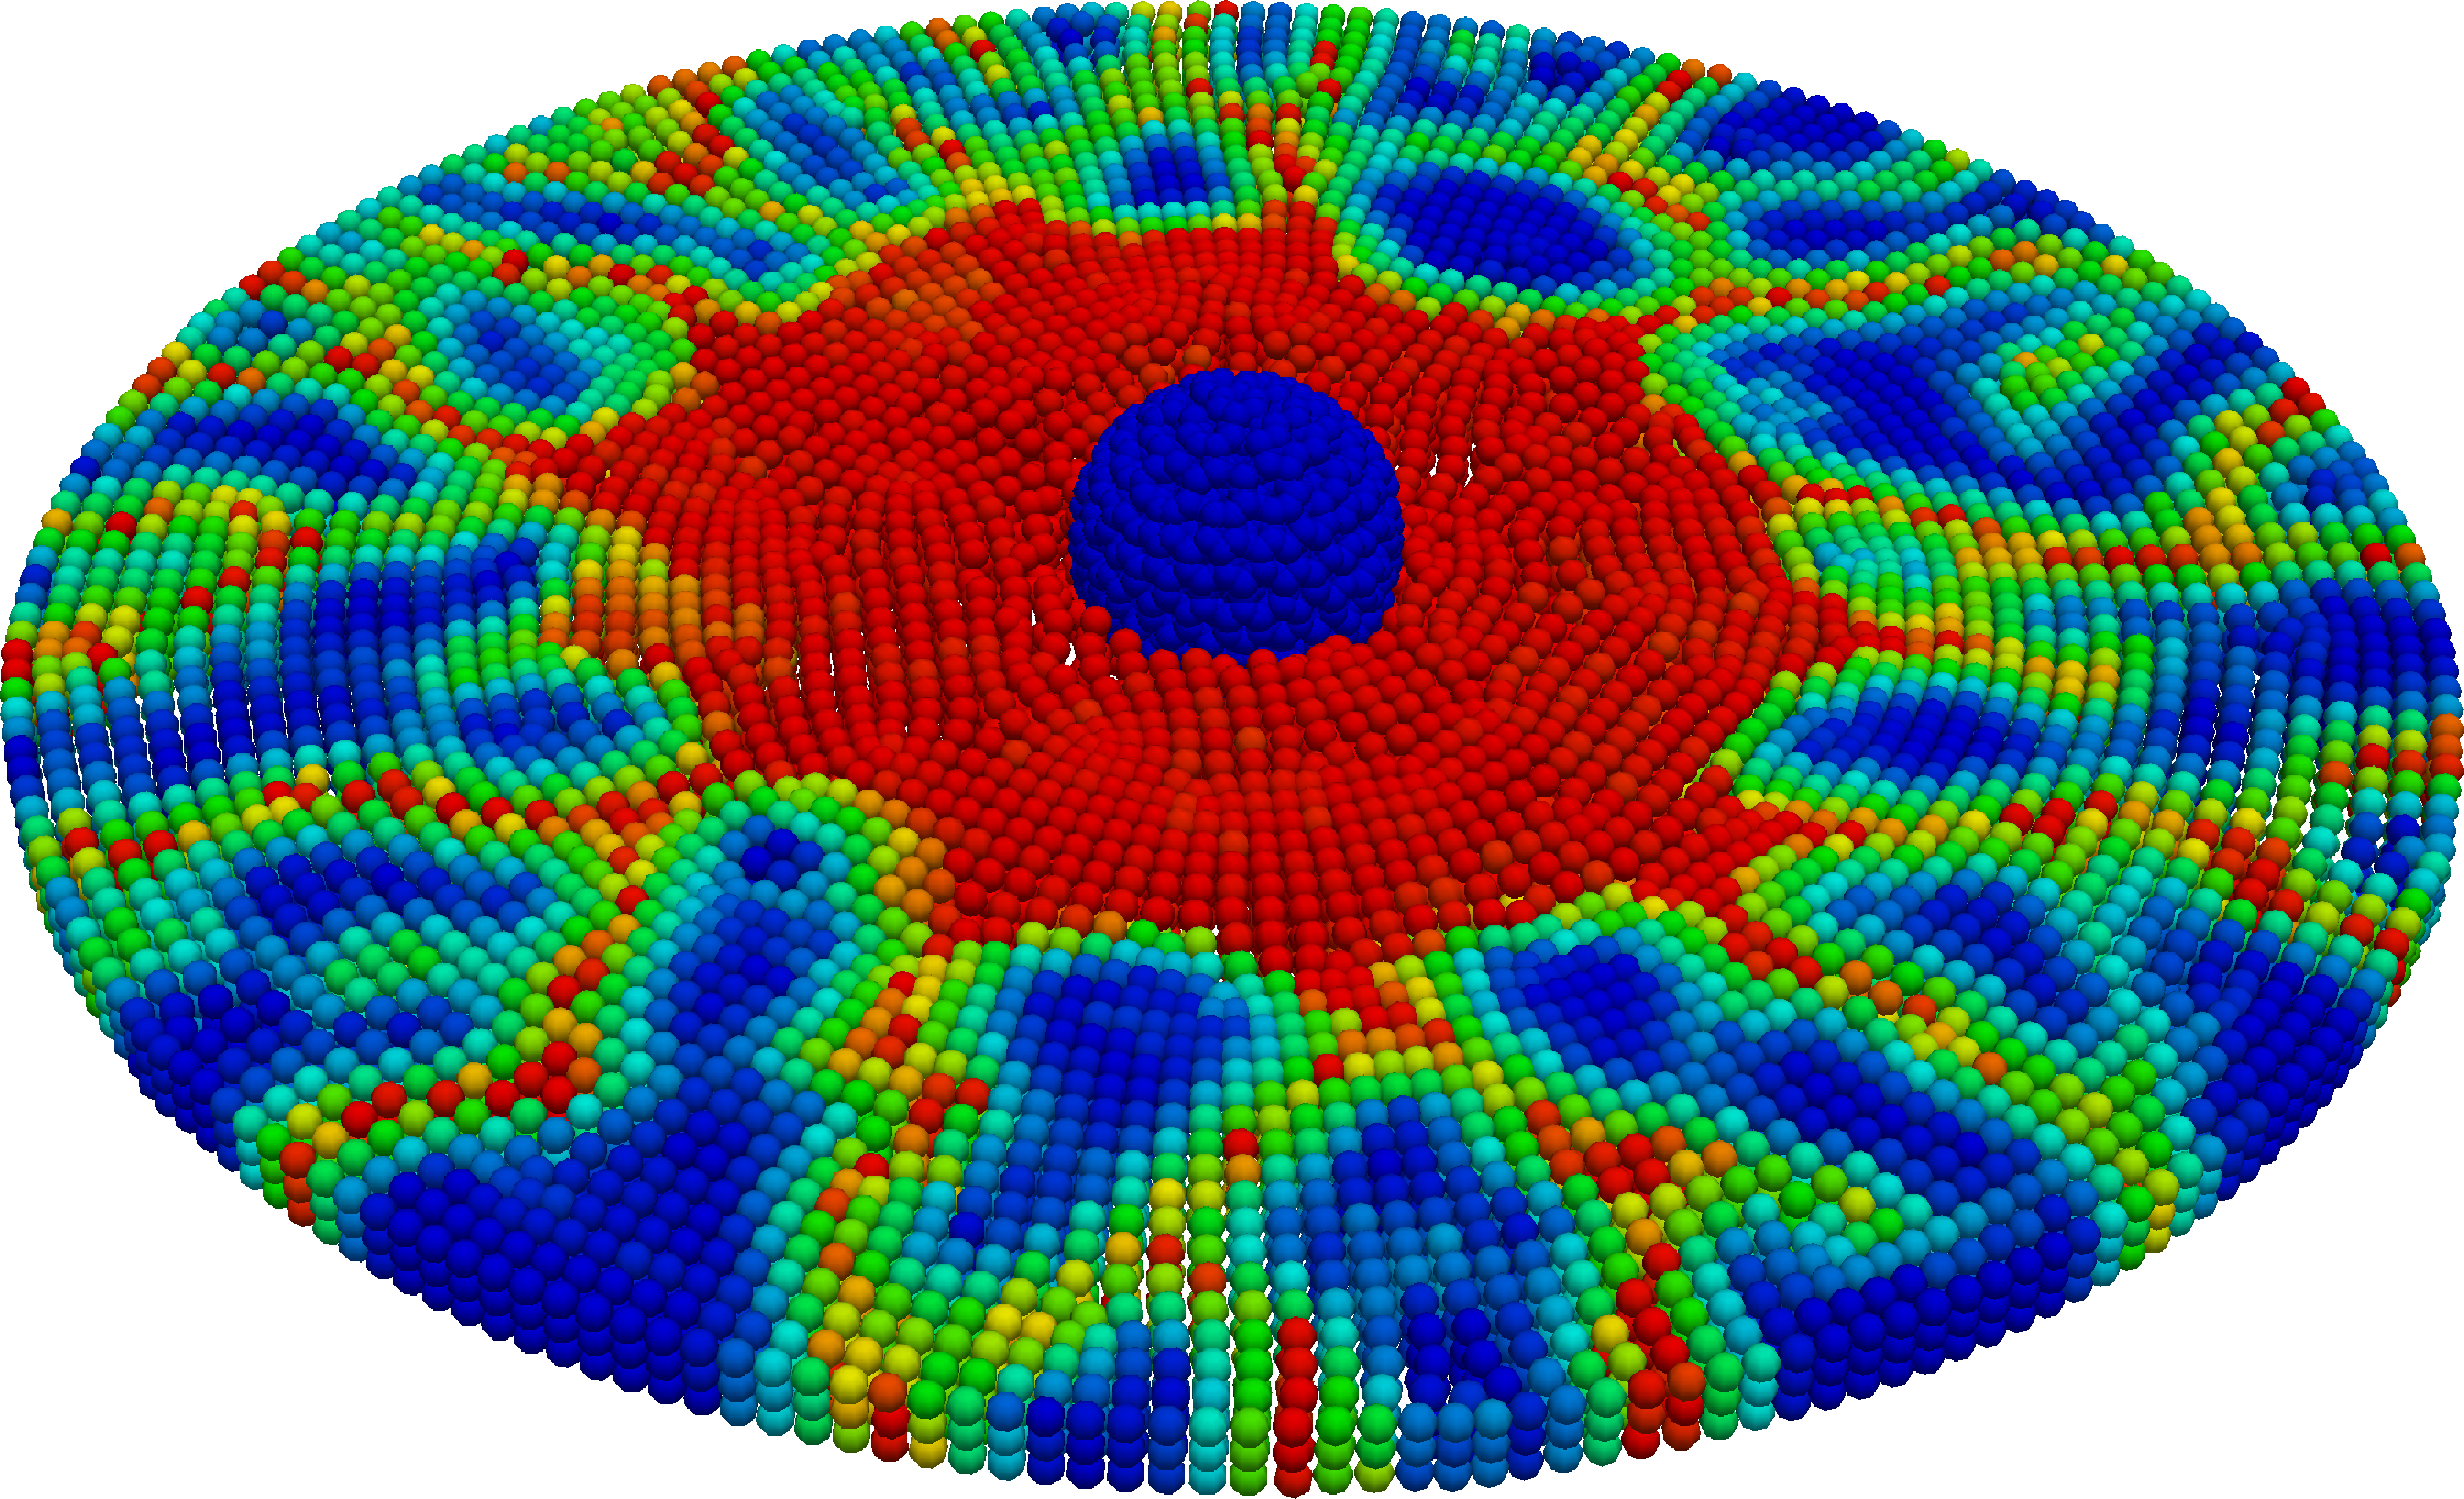
\includegraphics[width=0.7\linewidth]{Figures/Examples/Disk_Impact/Peridigm_Disk_Impact_47_Damage_ct}};
% Relative node positioning to picture
\node[anchor=east] (impactorlabel) at ($(image.west)       + (-0.5cm, 0.5)$) {Impactor};
\node[anchor=west] (disklabel)     at ($(image.south east) + ( 0.5cm,0.5)$) {Disk};
% Figure scope
\begin{scope}[
  x={(image.south east)},
  y={(image.north west)},
]
  % Some label
  \node [
    align=center,
    fill=white,
    rounded corners,
    anchor=south west
  ] at (0.05,0.1) {%
    A label with a manual linebreak\\%
    thanks to align option\\%
    using picture coordinate system%
  };
  % Some label
  \node [
    text width=3cm,
    align=center,
    fill=white,
    rounded corners
  ] at (0.75,0.65) {%
    A label with automatic linebreaks%
    thanks to text width option%
    using picture coordinate system%
  };
  % Arrows
  \draw[-latex, gray]   (impactorlabel.east) -- (0.5,0.65);
  \draw[-stealth, gray] (disklabel.west)     -- (0.9,0.2);
  % Highlight
  \draw[red,ultra thick,rounded corners] (0.72,0.05) rectangle (0.88,0.15);
  % Help grid and labels
  \draw[help lines,xstep=.1,ystep=.1] (0,0) grid (1,1);
  \foreach \x in {0,1,...,9} {\node [anchor=north] at (\x/10,0) {0.\x};}
  \foreach \y in {0,1,...,9} {\node [anchor=east]  at (0,\y/10) {0.\y};}
\end{scope}
% Outside label
\end{tikzpicture}
\caption{Labels on external picture example}
\label{fig:Labels_on_external_picture}
\end{figure}

The source code to create this figure is shown in section \ref{sec:Labels_on_external_graphics_Example} and can be downloaded from within this document.

% \newpage
\levelstay{Use animations in beamer presentations}
\label{sec:Use_LaTeX_Animations_in_Beamer}

Prerequisite for the following points is the creation of an animation in \marktool{\paraviewname}. The animation is saved as an avi-video file.

\begin{itemize}[noitemsep]
\item \marktool{\paraviewname} video animations can not be imported directly to \LaTeX{} beamer presentations using the following approach based on the \verb+media9+-package
\item Convert the avi-video to a mp4-video with H.264-video- and mp3-audio-codec, e.g. with \href{http://www.videolan.org/index.de.html}{VLC player}, see section \ref{sec:Use_Animations_VLC}
\item Add \lstinline[style=inlinetexstyle]+\usepackage{media9}+ to the preamble of your \LaTeX{} document
\item Embed the video using the script from section \ref{sec:Beamer_Video}
\item Play the video with Acrobat Reader under Windows
\end{itemize}

\input{Figures/LaTeX/Use_Videos_inside_Figure}

% \newpage
\levelstay{Create charts from result files}

This needs \lstinline[style=inlinetexstyle]+\usetikzlibrary{spy}+ in the preamble of the document.

First, the common \verb+pgfplotsset+ for the plots are created. These are shown in section \ref{sec:Nice_Charts_plotssets}. Add the code somewhere in your document. It can be in the preamble or right before the figures. 

Afterwards, the figure code can be included. The complete code is shown in section \ref{sec:Nice_Charts_Figure}. The result is shown in figure \ref{fig:Chart_Example}.

\begin{figure}[htbp]
\centering
\tikzexternalenable
\tikzsetnextfilename{Chart_Example}

\begin{tikzpicture}[%
  spy using outlines={%
    rectangle,                                % Spy form
    rounded corners,                          % Spy edge shape
    magnification=4,                          % Magnification factor
    height=0.6cm,                             % Height in original chart
    width=1.25cm,                             % Width in original chart
    dashed,                                   % Dashed line
    draw=gray,                                % Line color
    every spy on node/.append style={thick},  % Line style for spy
    connect spies,                            % Connect orig. & detail
    spy connection path={                     % Line style for spy connection
      \draw[thick] (tikzspyonnode) -- (tikzspyinnode);
    },
  }
]
  \begin{axis}[
    chart style,
    xlabel={Time [ms]},
    ylabel={Displacement [mm]},
  ]
    % Graph 1
    \addplot[
      gray,                                   % Plot color
      xaxis style,                            % Predefined style
    ] table [
      x expr=\thisrowno{0}*1000,              % Scale to ms
      y expr=\thisrowno{1}*1000,              % Scale to mm
    ]{Results/coord_disp_pd_nt100.txt};       % Input file
    \addlegendentry{Peridynamics}             % Legend entry
    % Graph 2
    \addplot[
      black,                                  % Plot color
      xaxis style,                            % Predefined style
    ] table [
      x expr=\thisrowno{0}*1000,              % Scale to ms
      y expr=\thisrowno{2}*1000,              % Scale to mm
    ]{Results/coord_disp_pd_nt100.txt};       % Input file
    \addlegendentry{Analytical}               % Legend entry
    % Spy 1
    \coordinate (spypoint1) at (axis cs:1.59,0.5);
    \coordinate (spyviewer1) at (axis cs:0.75,0.675);
    \spy[
      width=2.0cm,
      height=1.0cm,
    ] on (spypoint1) in node [
      fill=white,
      draw=gray,
      dashed
    ] at (spyviewer1);
    % Spy 2
    \coordinate (spypoint2) at (axis cs:4.76,0.5);
    \coordinate (spyviewer2) at (axis cs:3.92,0.675);
    \spy[
      width=2.0cm,
      height=1.0cm,
    ] on (spypoint2) in node [
      fill=white,
      draw=gray,
      dashed
    ] at (spyviewer2);
  \end{axis}
\end{tikzpicture}

\tikzexternaldisable
\caption{Comparison of analytical and peridynamic solution of wave in bar}
\label{fig:Chart_Example}
\end{figure}

Since result files can contain a lot of data and therefore exaggerate the use of \TeX{}-memory and compile time, consider externalization of the figure creation as explained in section \ref{sec:Externalize_Figure_Creation}.

% \newpage
\levelstay{Handling large result files in \protect\LaTeX}

\leveldown{Increase \TeX{}-memory}      \label{sec:Increase_TeX_Memory}

For large figures or plots of results using \verb+pgfplots+ the initial \TeX{} memory might be insufficient. A first possibility to solve that problem is to increase the \TeX{} memory.

\leveldown{MiKTeX on Windows}

\begin{itemize}[noitemsep]
\item Open a command prompt (cmd)
\item Type \colorbox{verbgray}{\lstinline[style=inlinetexstyle]+initexmf --edit-config-file pdflatex+} and press Enter
\item A file pops up in the editor
\item Add \colorbox{verbgray}{\lstinline[style=inlinetexstyle]+main_memory=8000000+} to the file
\item Save the file
\item Go back to the command prompt
\item Type \colorbox{verbgray}{\lstinline[style=inlinetexstyle]+initexmf --dump=pdflatex+} and press Enter
\item After completion, close the command prompt
\end{itemize}

\levelstay{TeXLive on Linux}

Untested:

\begin{itemize}[noitemsep]
\item Open a terminal
\item Type \colorbox{verbgray}{\lstinline[style=inlinetexstyle]+kpsewhich texmf.cnf+} and press Enter
\item This gives the path to the \verb+texmf.cnf+ file
\item Open the file
\item Change or add \colorbox{verbgray}{\lstinline[style=inlinetexstyle]+main_memory=8000000+} to the file
\item Save the file
\item Go back to the command prompt
\item Type \colorbox{verbgray}{\lstinline[style=inlinetexstyle]+sudo fmtutil-sys --all+} and press Enter
\item After completion, close the command prompt
\end{itemize}

Be aware that using this method you modify the official config file which will be overwritten in an update. Thus, you have to repeat this step after an update. A better and update-independent solution is to create a local \verb+texmf.cnf+-file and register it in the \TeX{} path variables

\levelup{Externalize TikZ- \& pgfplots-figure creation} \label{sec:Externalize_Figure_Creation}

Creation of \lstinline[style=inlinetexstyle]+TikZ+ or \lstinline[style=inlinetexstyle]+pgfplotsset+-figures can be quite memory and time consuming. The creation of these figures can be externalized to save time. This means the figure is compiled once and written to a graphics file (pdf, png, ...). The next \lstinline[style=inlinetexstyle]+pdflatex+ run re-uses the created figure. It is not re-created for each compilation.

To achieve the externalization you need to add the following code to your preamble in addition to \lstinline[style=inlinetexstyle]+\usepackage{pgfplots}+:

\begingroup
\lstset{breaklines = true}
\lstinputlisting[
  style=texstyle,
  caption=TikZ externalization code,
  label=lst:TikZ_externalize,
  ]{\peridoccommonpath/Preamble/Pref_Packages_TikZ_Externalization}
\endgroup

\ifpdf
You can \textattachfile[author=raed_ma, color=0 0 1]{\peridoccommonpath/Preamble/Pref_Packages_TikZ_Externalization}{download} the file from within this document.
\fi

Using one of the last two lines of the \verb+tikzset+ converts the pdf file of the figure created by \verb+pdflatex+ to a png file. It requires the installation of \href{http://www.imagemagick.org/script/index.php}{ImageMagick} which provides the \verb+convert+ command for ImageMagick version prior to 7 or \verb+magick+ for version 7 or newer. For this to work, the path to the ImageMagick binaries \verb+convert.exe+ or \verb+magick.exe+ must be added to the system \texttt{PATH} environment variable.

In case you want to externalize the creation of a single figure add the following:

\begin{texcode}
\tikzexternalenable                     �\lstcomment{\% Enable externalization}�
\tikzsetnextfilename{Chart_Example}     �\lstcomment{\% Figure file name}�

\begin{tikzpicture}[%
  spy using outlines={%
    rectangle,                                % Spy form
    rounded corners,                          % Spy edge shape
    magnification=4,                          % Magnification factor
    height=0.6cm,                             % Height in original chart
    width=1.25cm,                             % Width in original chart
    dashed,                                   % Dashed line
    draw=gray,                                % Line color
    every spy on node/.append style={thick},  % Line style for spy
    connect spies,                            % Connect orig. & detail
    spy connection path={                     % Line style for spy connection
      \draw[thick] (tikzspyonnode) -- (tikzspyinnode);
    },
  }
]
  \begin{axis}[
    chart style,
    xlabel={Time [ms]},
    ylabel={Displacement [mm]},
  ]
    % Graph 1
    \addplot[
      gray,                                   % Plot color
      xaxis style,                            % Predefined style
    ] table [
      x expr=\thisrowno{0}*1000,              % Scale to ms
      y expr=\thisrowno{1}*1000,              % Scale to mm
    ]{Results/coord_disp_pd_nt100.txt};       % Input file
    \addlegendentry{Peridynamics}             % Legend entry
    % Graph 2
    \addplot[
      black,                                  % Plot color
      xaxis style,                            % Predefined style
    ] table [
      x expr=\thisrowno{0}*1000,              % Scale to ms
      y expr=\thisrowno{2}*1000,              % Scale to mm
    ]{Results/coord_disp_pd_nt100.txt};       % Input file
    \addlegendentry{Analytical}               % Legend entry
    % Spy 1
    \coordinate (spypoint1) at (axis cs:1.59,0.5);
    \coordinate (spyviewer1) at (axis cs:0.75,0.675);
    \spy[
      width=2.0cm,
      height=1.0cm,
    ] on (spypoint1) in node [
      fill=white,
      draw=gray,
      dashed
    ] at (spyviewer1);
    % Spy 2
    \coordinate (spypoint2) at (axis cs:4.76,0.5);
    \coordinate (spyviewer2) at (axis cs:3.92,0.675);
    \spy[
      width=2.0cm,
      height=1.0cm,
    ] on (spypoint2) in node [
      fill=white,
      draw=gray,
      dashed
    ] at (spyviewer2);
  \end{axis}
\end{tikzpicture}
     �\lstcomment{\% Path to figure}�
\tikzexternaldisable                    �\lstcomment{\% Disable externalization}�
\end{texcode}

Beware, if you make changes to a figure you have to delete the present figure file before compiling your document. Otherwise, the update will not be effective because the old figure is re-used.

\levelup{Tips and tricks with Biber}

%%%%%%%%%%%%%%%%%%%%%%%%%%%%%%%%%%%%
% Bibliography                     %
%%%%%%%%%%%%%%%%%%%%%%%%%%%%%%%%%%%%

\printbibliography

%%%%%%%%%%%%%%%%%%%%%%%%%%%%%%%%%%%%
% Index                            %
%%%%%%%%%%%%%%%%%%%%%%%%%%%%%%%%%%%%

% \printindex[\idxKeywordName]

%%%%%%%%%%%%%%%%%%%%%%%%%%%%%%%%%%%%
% Appendix                         %
%%%%%%%%%%%%%%%%%%%%%%%%%%%%%%%%%%%%

%%%%%%%%%%%%%%%%%%%%%%%%%%%%%%%%%%%%
% Header                           %
%%%%%%%%%%%%%%%%%%%%%%%%%%%%%%%%%%%%
% 
% Revisions: 2017-04-10 Martin Rädel <martin.raedel@dlr.de>
%                       Initial draft
%               
% Contact:   Christian Willberg,  christian.willberg@dlr.de
%            DLR Composite Structures and Adaptive Systems
%          
%                                 __/|__
%                                /_/_/_/  
%            www.dlr.de/fa/en      |/ DLR
% 
%%%%%%%%%%%%%%%%%%%%%%%%%%%%%%%%%%%%
% Content                          %
%%%%%%%%%%%%%%%%%%%%%%%%%%%%%%%%%%%%
\begin{appendices}
  %%%%%%%%%%%%%%%%%%%%%%%%%%%%%%%%%%%%
% Header                           %
%%%%%%%%%%%%%%%%%%%%%%%%%%%%%%%%%%%%
% 
% 
% 
% Revisions: 2017-04-10 Martin R�del <martin.raedel@dlr.de>
%                       Initial draft
%               
% Contact:   Martin R�del,  martin.raedel@dlr.de
%            DLR Composite Structures and Adaptive Systems
%          
%                                 __/|__
%                                /_/_/_/  
%            www.dlr.de/fa/en      |/ DLR
% 
%%%%%%%%%%%%%%%%%%%%%%%%%%%%%%%%%%%%
% Content                          %
%%%%%%%%%%%%%%%%%%%%%%%%%%%%%%%%%%%%

\chapter{This document}
\setcounter{currentlevel}{6}

\leveldown{Repository}

%%%%%%%%%%%%%%%%%%%%%%%%%%%%%%%%%%%%
% Header                           %
%%%%%%%%%%%%%%%%%%%%%%%%%%%%%%%%%%%%
% 
% Revisions: 2017-04-10 Martin R�del <martin.raedel@dlr.de>
%                       Initial draft
%               
% Contact:   Martin R�del,  martin.raedel@dlr.de
%            DLR Composite Structures and Adaptive Systems
%          
%                                 __/|__
%                                /_/_/_/  
%            www.dlr.de/fa/en      |/ DLR
% 
%%%%%%%%%%%%%%%%%%%%%%%%%%%%%%%%%%%%
% Content                          %
%%%%%%%%%%%%%%%%%%%%%%%%%%%%%%%%%%%%

This document is part of the \reponame{} repository. The complete repository can be found at:

\href{\repoaddress}{\repoaddress}

% \levelstay{Development plans}
% 
% %%%%%%%%%%%%%%%%%%%%%%%%%%%%%%%%%%%%
% Header                           %
%%%%%%%%%%%%%%%%%%%%%%%%%%%%%%%%%%%%
% 
% Revisions: 2017-04-10 Martin R�del <martin.raedel@dlr.de>
%                       Initial draft
%               
% Contact:   Martin R�del,  martin.raedel@dlr.de
%            DLR Composite Structures and Adaptive Systems
%          
%                                 __/|__
%                                /_/_/_/  
%            www.dlr.de/fa/en      |/ DLR
%
%%%%%%%%%%%%%%%%%%%%%%%%%%%%%%%%%%%%
% Content                          %
%%%%%%%%%%%%%%%%%%%%%%%%%%%%%%%%%%%%

% \chapter{Development plan}
% \setcounter{currentlevel}{6}

An issue tracker has been setup:

\href{https://free-redmine.saas-secure.com/projects/peridox}{https://free-redmine.saas-secure.com/projects/peridox}

Contact the author of this document about information how to access and edit the issue tracker.

% \begin{table}[htbp]
% \caption{Requirement list}
% \label{tab:requirementList}
% \begin{tabularx}{\linewidth}{XXX}
% \toprule
% What&Why & Where \\
% \midrule
% Read coordinate system&read local coordinate systems from exodus&io/Peridigm\_DiscretizationFactory.cpp;io/Peridigm\_ExodusDiscretization.cpp	\\
% local material coordinate transformation&describe anisotropic material accurately &material/Peridigm\_MaterialFactory.cpp; core/\\
% delete bonds in correspondence material&simulate crack propagation with correspondence material&material/Peridigm\_MaterialFactory.cpp	\\
% \bottomrule
% \end{tabularx}
% \end{table}


\levelstay{Typesetting}

%%%%%%%%%%%%%%%%%%%%%%%%%%%%%%%%%%%%
% Header                           %
%%%%%%%%%%%%%%%%%%%%%%%%%%%%%%%%%%%%
% 
% Revisions: 2017-04-10 Martin R�del <martin.raedel@dlr.de>
%                       Initial draft
%               
% Contact:   Martin R�del,  martin.raedel@dlr.de
%            DLR Composite Structures and Adaptive Systems
%          
%                                 __/|__
%                                /_/_/_/  
%            www.dlr.de/fa/en      |/ DLR
% 
%%%%%%%%%%%%%%%%%%%%%%%%%%%%%%%%%%%%
% Content                          %
%%%%%%%%%%%%%%%%%%%%%%%%%%%%%%%%%%%%


This document was originally typeset using the documentclass \texttt{dlrreprt} from the DLR-internal RM-\LaTeX{} package.

The RM-\LaTeX{} package is not publicly available. Therefore, this document is compatible with a bootstrap-version of the documentclass, called \texttt{bootstrap\_dlrreprt}. \texttt{bootstrap\_dlrreprt} class is part of this repository.

The compilation is performed with \verb+pdflatex+ with the following options:

\begingroup
\lstset{breaklines=true}
\begin{texcode}
pdflatex --shell-escape -synctex=1 -interaction=nonstopmode %source --extra-mem-top=60000000
\end{texcode}
\endgroup

The bibliography is compiled with \verb+biber+. The glossary must be compiled with makeindex or, for \windowsosname{}, the included batch-script may be used. The keyword index is created automatically.

The general compilation order is:

\verb+pdflatex+ $\rightarrow$
\verb+biber+ $\rightarrow$
\verb+makeindex+ $\rightarrow$
\verb+pdflatex+ $\rightarrow$
\verb+pdflatex+
\end{appendices}

\input{\peridoccommonpath/Sections/License_BSDDL_Text}


\end{document} 